\documentclass[oneside]{article}

\usepackage{blindtext} % Package to generate dummy text throughout this template 
\usepackage{graphicx} % FKM: for figures
\usepackage{color} % FKM: for colored text
\usepackage{float} % FKM: for forcing figure placement
\usepackage[breakable]{tcolorbox} % FKM: for text box
\usepackage{enumerate} % FKM: for bullet point lists
\usepackage{setspace} % FKM: line spacing
\usepackage[margin=1in]{geometry} % FKM: margins


\usepackage[sc]{mathpazo} % Use the Palatino font
\usepackage[T1]{fontenc} % Use 8-bit encoding that has 256 glyphs
% \linespread{1.05} % Line spacing - Palatino needs more space between lines
\usepackage{microtype} % Slightly tweak font spacing for aestheticsgins
\usepackage[small,labelfont=bf,up,up]{caption} % Custom captions under/above floats in tables or figures
\usepackage{booktabs} % Horizontal rules in tables
\usepackage{amsmath} % Text in equations
\usepackage{titlesec} % Allows customization of titles
\usepackage{titling} % Customizing the title section
\usepackage[hidelinks]{hyperref} % For hyperlinks in the PDF
\usepackage{tikz}
\usepackage{standalone}

\usepackage{subcaption} % for subfigures side by side
\captionsetup[subfigure]{singlelinecheck=false} % to put (a) and (b) at the top-left of subfigures

\usepackage[shortlabels]{enumitem} % customized lists (shortlabels
                                % necessary to have i., ii., etc., in enumerate)
\setlist[itemize]{noitemsep} % Make itemize lists more compact

\usepackage{abstract} % Allows abstract customization
\renewcommand{\abstractnamefont}{\normalfont\bfseries} % Set the "Abstract" text to bold
\renewcommand{\abstracttextfont}{\normalfont\small\itshape} % Set the abstract itself to small italic text

\usepackage{fancyhdr} % Headers and footers
\pagestyle{fancy} % All pages have headers and footers
\fancyhead{} % Blank out the default header
\fancyfoot{} % Blank out the default footer
\fancyhead[C]{Authors et al. $\bullet$ August 2018 $\bullet$ bio{\color{red}R}$\chi$ve} % Custom header text
\fancyfoot[RO,LE]{\thepage} % Custom footer text



\usepackage{natbib}
\bibliographystyle{apalike}

\usepackage{libertine}

\setlength\columnsep{20pt}

%----------------------------------------------------------------------------------------
%	TITLE SECTION
%----------------------------------------------------------------------------------------

\setlength{\droptitle}{-4\baselineskip} % Move the title up

%\pretitle{\begin{center}\Huge\bfseries} % Article title formatting
%\posttitle{\end{center}} % Article title closing formatting

\title{How to validate a Bayesian model} % Article title
%LM: strictly speaking, we're 'validating' the inference machinery.
%% Validating a model involves epistemic considerations that are, as far as I understand, outside the scope of this paper.
\author{\textsc{F\'{a}bio K. Mendes$^{1*}$}, \textsc{Remco Bouckaert$^{2*}$},\\
\textsc{Christiaan Swanepoel$^{2}$}, \textsc{Alexei J. Drummond$^{1,2}$} \\
\small $^1$School of Biological Sciences, The University of Auckland\\
\small $^2$School of Computer Science, The University of Auckland\\
\small
\href{mailto:f.mendes@auckland.ac.nz}{Corresponding authors$^*$:
  f.mendes@auckland.ac.nz, remco@cs.auckland.ac.nz}
% \href{mailto:f.mendes@auckland.ac.nz}{another.email@auckland.ac.nz}
%\and % Uncomment if 2 authors are required, duplicate these 4 lines if more
%\textsc{Jane Smith}\thanks{Corresponding author} \\[1ex] % Second author's name
%\normalsize University of Utah \\ % Second author's institution
%\normalsize \href{mailto:jane@smith.com}{jane@smith.com} % Second author's email address
}
\date{\today} % Leave empty to omit a date
\renewcommand{\maketitlehookd}{%
\begin{abstract}
  \noindent Biology has become a highly mathematical discipline in
  which probabilistic models play a central role,
  and as a result research in the biological sciences is now dependent on
  computational tools capable of carrying out complex analyses.
  These tools must not only be efficient, but also correctly
  implemented.
  Both goals are difficult to achieve for several reasons, such as the
  multidisciplinary nature of method development, and a still
  embrionic literature on good software development and statistical
  practices aimed at professionals from disparate fields.
  Here we provide guidelines for the validation of probabilistic model
  implementations, focusing on Bayesian approaches.
  This manuscript summarizes good practices for assessing the correctness of
  simulation and inference procedures under a model, and is available in
  the traditionally static print version as well as in a reproducible and
  executable form.
\end{abstract}
\centering [Probabilistic models, Bayesian models, model validation, coverage]
}

%----------------------------------------------------------------------------------------

\doublespacing

\begin{document}

% Print the title
\maketitle

%----------------------------------------------------------------------------------------
%	ARTICLE CONTENTS
%----------------------------------------------------------------------------------------

\section*{Introduction}
The last two decades have seen the biological sciences undergo a major revolution.
Critical technological innovations such as the advent of massive
parallel sequencing and the accompanying improvements in computational
power and storage have flooded biology with unprecedented amounts of
data ripe for analysis.
Not only has intraspecific data from multiple individuals allowed
progress in fields like medicine and epidemiology
\citep[e.g.,][]{1000g,humanmicrobiome,neafsey15}, population genetics
\citep[e.g.,][]{lynch07,lack16,demanuel16} and disease ecology
\citep[e.g.,][]{rosenblum13,bates18}, but now a large number of species
across the tree of life have had their genomes sequenced, furthering
our understanding of species relationships and diversification
\citep[e.g.,][]{martin13,brawand14,jarvis14,novikova16,pease2016,kawahara19,upham19}.
However, as the old adage goes, with great power comes great
responsibility: never has the data available to the average biologist
been so abundant, but also never has one been so aware of both its
complexity and the necessary care needed to analyze it.
Almost on par with with data accumulation is the rate at which new
computational tools are being proposed, as evidenced by journals
entirely dedicated to method advances, methodological sections in
biological journals, and computational biology degrees being offered
by institutions around the world.

One extreme case is the discipline of evolutionary biology (on which
we focus our attention).
While it could be said that many decade-old questions and hypotheses
in evolutionary biology have aged well and stood up the test of time
(e.g., the Red Queen hypothesis,
\citealt{vanvalen73,lively87,morran11,gibson15}; the
Bateson-Dobzhansky-Muller model,
\citealt{dob36,muller40,hopkins12,roda17}), data analysis practices
have changed drastically in recent years, to the point they would
likely seem exotic and obscure to an evolutionary biologist active
forty years ago.
In particular, evolutionary biology has become highly statistical,
with the development and utilization of models now being commonplace.

Models are employed in the sciences for many reasons, and fall within
a biological abstraction continuum \citep{servedio14}, going from
fully verbal, highly abstract models (e.g., \citealt{vanvalen73}),
through proof-of-concept models that formalize verbal models (e.g.,
\citealt{maynard78,reinhold99,mendes18}), to models that
interact directly with data through explicit mathematical
functions \citep{yule24,felsenstein73,hky,hudson90}).
Within the latter category, probabilistic models have seen a sharp surge
in popularity within evolutionary biology, in conjunction
with computational tools implementing them.

Despite the increasing pervasiveness of probabilistic models in the
biological sciences, tools implementing such models show large
variation not only with respect to code quality (from a software engineering
perspective), but also correctness \citep{darriba18}.
This is unsurprising given the multidisciplinary nature of model and method
development, and the challenges inherent to software research funding
\citep{siepel19}.
The bioinformatics community is thus in dire need of resources that
provide guidance for code improvement and validation.

Here, we summarize best practices in probabilistic model validation for method
developers, with an emphasis on Bayesian methods.
This manuscript is also presented in a reproducible and executable version
[LINK TO STENCILA VERSION], and is accompanied by code examples for these practices
(with the BEAST 2 platform as a reference; \citealp{beast25}).

% \begin{figure}
%   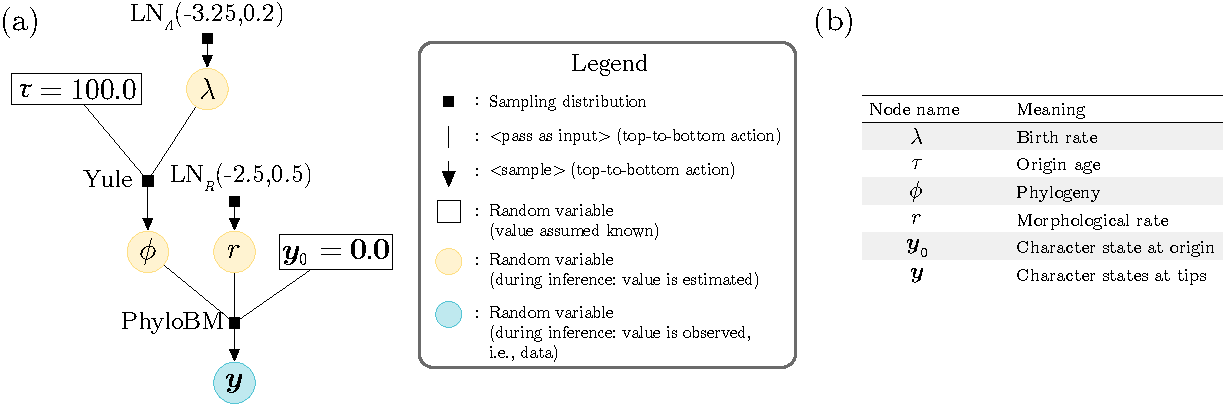
\includegraphics[width=\linewidth]{fig1}
%   \caption{Hemiplasy on species trees and gene trees.
%     Panel (a) shows substitutions that occur on each of the two discordant gene trees, and the corresponding site patterns produced.
%     (b) Incorrectly inferred convergent substitutions (from the site patterns produced in [a]) when analyses are conducted on the species tree topology.
%     (c) Incorrectly inferred convergent substitutions when analyses are conducted on the CDS tree (discordant tree topology 2).}
%   \label{fig:1}
% \end{figure}

%------------------------------------------------

\section*{Probabilistic models}

Probabilistic models mathematically formalize natural phenomena
having an element of randomness.
This is done through probability distributions describing both the observed
empirical data -- seen as the result of one or more random
instantiations of the modeled process -- as well the model parameters,
which abstract relevant, but usually unknown aspects
of the phenomenon at hand.
The historical, stochastic, and highly dimensional nature of evolutionary
processes makes the utility of probabilistic models in evolutionary
biology self-evident. 

The central component of a probabilistic model, $\text{P}(D|\theta)$,
describes the probability distribution over the data given the model
parameters.
This probability mass function (pmf; or its continuous
countepart, the probability density function $f(D|\theta)$) is sometimes
referred to as the likelihood function.
As illustrated in the next sections, probabilistic models can be
hierarchical, in which case there may be several likelihood functions.
% (Fig. \ref{fig:graphmodel}).
In a frequentist statistical framework, $\text{P}(D|\theta)$ is the sole
component of a probabilistic model, and is maximized across parameter ($\theta$) space during parameter estimation and model comparison.

In the present study we focus on Bayesian inference, however, 
where a probabilistic model $\mathcal{M}$ defines a posterior probability
distribution for its parameters, $\text{P}(\theta|D) =
\frac{\text{P}(D|\theta)\text{P}(\theta)}{\text{P}(D)}$.
Here, our prior inferences or beliefs about the natural world -- represented by
the prior distribution $\text{P}(\theta)$ -- are confronted and updated by
the data through the likelihood function (or multiple likelihood functions).
$\text{P}(D) = \int_\theta \text{P}(D|\theta)\text{P}(\theta)d\theta$, the
probability of the data, is also known as the marginal likelihood or the model
evidence.
Crucially, a Bayesian model includes a prior, $\text{P}(\theta)$:
when models are compared, for example, $\text{P}(\theta)$ needs to be taken
into account when computing the model evidence $\text{P}(D)$.

Models routinely used in evolutionary biology are often characterized by
continuous parameters, and are normally complex enough to preclude
analytical solutions for the posterior density $f(\theta|D)$, mainly
due to the intractability of the integral appearing in the marginal
likelihood.
In those cases, one can make use of the fact that $f(D)$
is a constant that can be ignored (i.e., $f(\theta|D)
\propto f(\theta|D)f(\theta)$), and use 
techniques like Markov chain Monte Carlo (MCMC) to sample the posterior
distribution.
This is because the MCMC algorithm that generates the Markov chain,
called the Metropolis-Hastings \citep{metropolis53,mh} algorithm, only requires the
posterior to be evaluated up to a constant.

In practice, the Metropolis-Hastings algorithm samples the posterior
distribution (also referred to as the ``target'' distribution) by means of a
transition mechanism. 
If the proposal distribution generated by this mechanism is
irreducible, positive recurrent, and aperiodic, and the resulting
chain is long enough, then the sampled posterior distribution will approximate
the target distribution $f(\theta|D)$ \citep{smith93,tierney94,gelman}.

We will spend time considering MCMC in particular as it is the commonly
chosen technique for obtaining $f(\theta|D)$ under an implementation of
model $\mathcal{M}$.
A thorough validation effort thus entails verifying the
correctness of (i) the model (i.e., $f(D|\theta)f(\theta)$), and (ii)
the components involved in the MCMC transition mechanism.
We note that the latter are not part of the model, however, and it is 
possible to sample $f(\theta|D)$ with other techniques such as importance
sampling, Hamiltonian Monte Carlo \citep{hmc}, or even by converting the
sampling problem into an optimization one \citep[e.g.,][]{zhang18}.

Finally, we stress that we are interested in practices for verifying model
\emph{correctness}.
There are other tests employed to ensure that a particular MCMC analysis
is converging as anticipated.
Determining that one or more independent Markov chains converged on very
similar posterior distributions is not a correctness test, as those
distributions might be very different from the target distribution.

\subsection*{Validating a Bayesian model}

\subsubsection*{Validating the simulator, $S[\mathcal{M}]$}\label{verify-correctness-of-simulator-implementation}

When a probabilistic model $\mathcal{M}$ is implemented for the first
time, a simulator $S[\mathcal{M}]$ must be devised and itself
validated before we can validate an inferential engine $I[\mathcal{M}]$.
It is $I[\mathcal{M}]$ that will be employed by users in empirical
analyses.
A simulator conventionally requires a parameter value as input (i.e.,
a $\theta$ value, where $\boldsymbol{\theta}$ might represent more than one
parameter), or a prior distribution on those values,
$f(\boldsymbol{\theta})$. 
The simulator then outputs a sample of random variable(s), which
for hierarchical models will include not only an instantiation of data
$\text{D}$, but also of a subset of the parameters in
$\boldsymbol{\theta}$.

In the case of hierarchical models, it is sometimes useful
to consider $S[\mathcal{M}]$ as a collection of component
simulators, each characterized by a different sampling distribution.
In figure X, for example, $S[\mathcal{M}]$ can be seen as an ensemble
comprised by (i) $S[f(\boldsymbol{\theta})]$ (where $\boldsymbol{\theta} = \{\lambda, r, r_m,
y_0\}$), which jointly simulates all parameters in $\boldsymbol{\theta}$,
(ii) $S[f(\Phi|\lambda)]$, which simulates a Yule tree $\Phi$, (iii)
$S[f(\mathbf{A}|\Phi,r)]$, which simulates a multiple sequence
alignment $\mathbf{A}$, and (iv) $S[f(\mathbf{M}|\Phi,r_m,y_0])$,
which simulates a continuous character vector $\mathbf{M}$ for all
species in $\Phi$.
Being able to isolate the building blocks of a hierarchical model simulator 
helps divide and conquer the validation task, especially when some, but
not all of the sampling distributions are well-known parametric distributions,
or when they result from well characterized stochastic processes (see below).

One way of validating a probabilistic model simulator is by 
sampling a large number of points, calculating summary statistics from the
sample, and comparing those statistics to either their true value
counterparts (i.e., the values used as input in the simulation), or to
their analytical expectations.
In Box 1, we illustrate this procedure for a known parametric distribution,
the multivariate normal distribution characterizing the phylogenetic
Brownian motion model \citep{felsenstein73}.

\vspace{.5cm}

% Start: BM BOX
\begin{tcolorbox}[breakable, width=\textwidth, colback=gray!10, boxrule=0pt,
  title=Box 1: Models characterized by well-known parametric distributions, fonttitle=\bfseries]
  \small 
  One commonly used model in macroevolution for the study
of continuous traits is the phylogenetic Brownian motion model (``PhyloBM'' in Fig. X;
\citealt{felsenstein73}).
The pdf characterizing this model's sampling distribution is in fact
the pdf of the multivariate normal (MVN) probability distribution:

\begin{equation}
  \begin{split}
    \text{log }f(\mathbf{y} \mid \boldsymbol{y_0}, r, \boldsymbol{T}) = -\frac{1}{2} \Big[ n\text{log}(2\pi) + \text{log}|r \boldsymbol{T}| \Big] & \\
    -\frac{1}{2} \Big[ (\mathbf{y} - \boldsymbol{y_0})^T (r \boldsymbol{T})^{-1} (\mathbf{y} - \boldsymbol{y_0}) \Big],
  \label{eq:bm}
  \end{split}
\end{equation}

\noindent where $\mathbf{y}$ corresponds to the observed trait values representing
$n$ species, $\boldsymbol{y_0}$ is the trait value at the root of the tree, $r$ is the variance
of the process (also known as the evolutionary rate, and sometimes represented by
$\sigma^2$), and $r\boldsymbol{T}$ is the variance-covariance matrix.
$\boldsymbol{T}$ is a matrix whose elements are deterministically defined by tree
$\Phi$'s branch lengths; see Fig. 1 below).

\vspace{.25cm}
The probability density function in equation \ref{eq:bm} describes the distribution
that would result from an infinite number of BM ``experiments'' (each experiment
being non-mean-reverting, and representing an independent evolutionary trajectory).
Under this model $\boldsymbol{\theta} = \{\boldsymbol{y_0}, r, \boldsymbol{T}\}$ and $D = \{\mathbf{y}\}$
(but note that sometimes researchers treat $\Phi$ and consequently $\boldsymbol{T}$ as
data).

\begin{center}
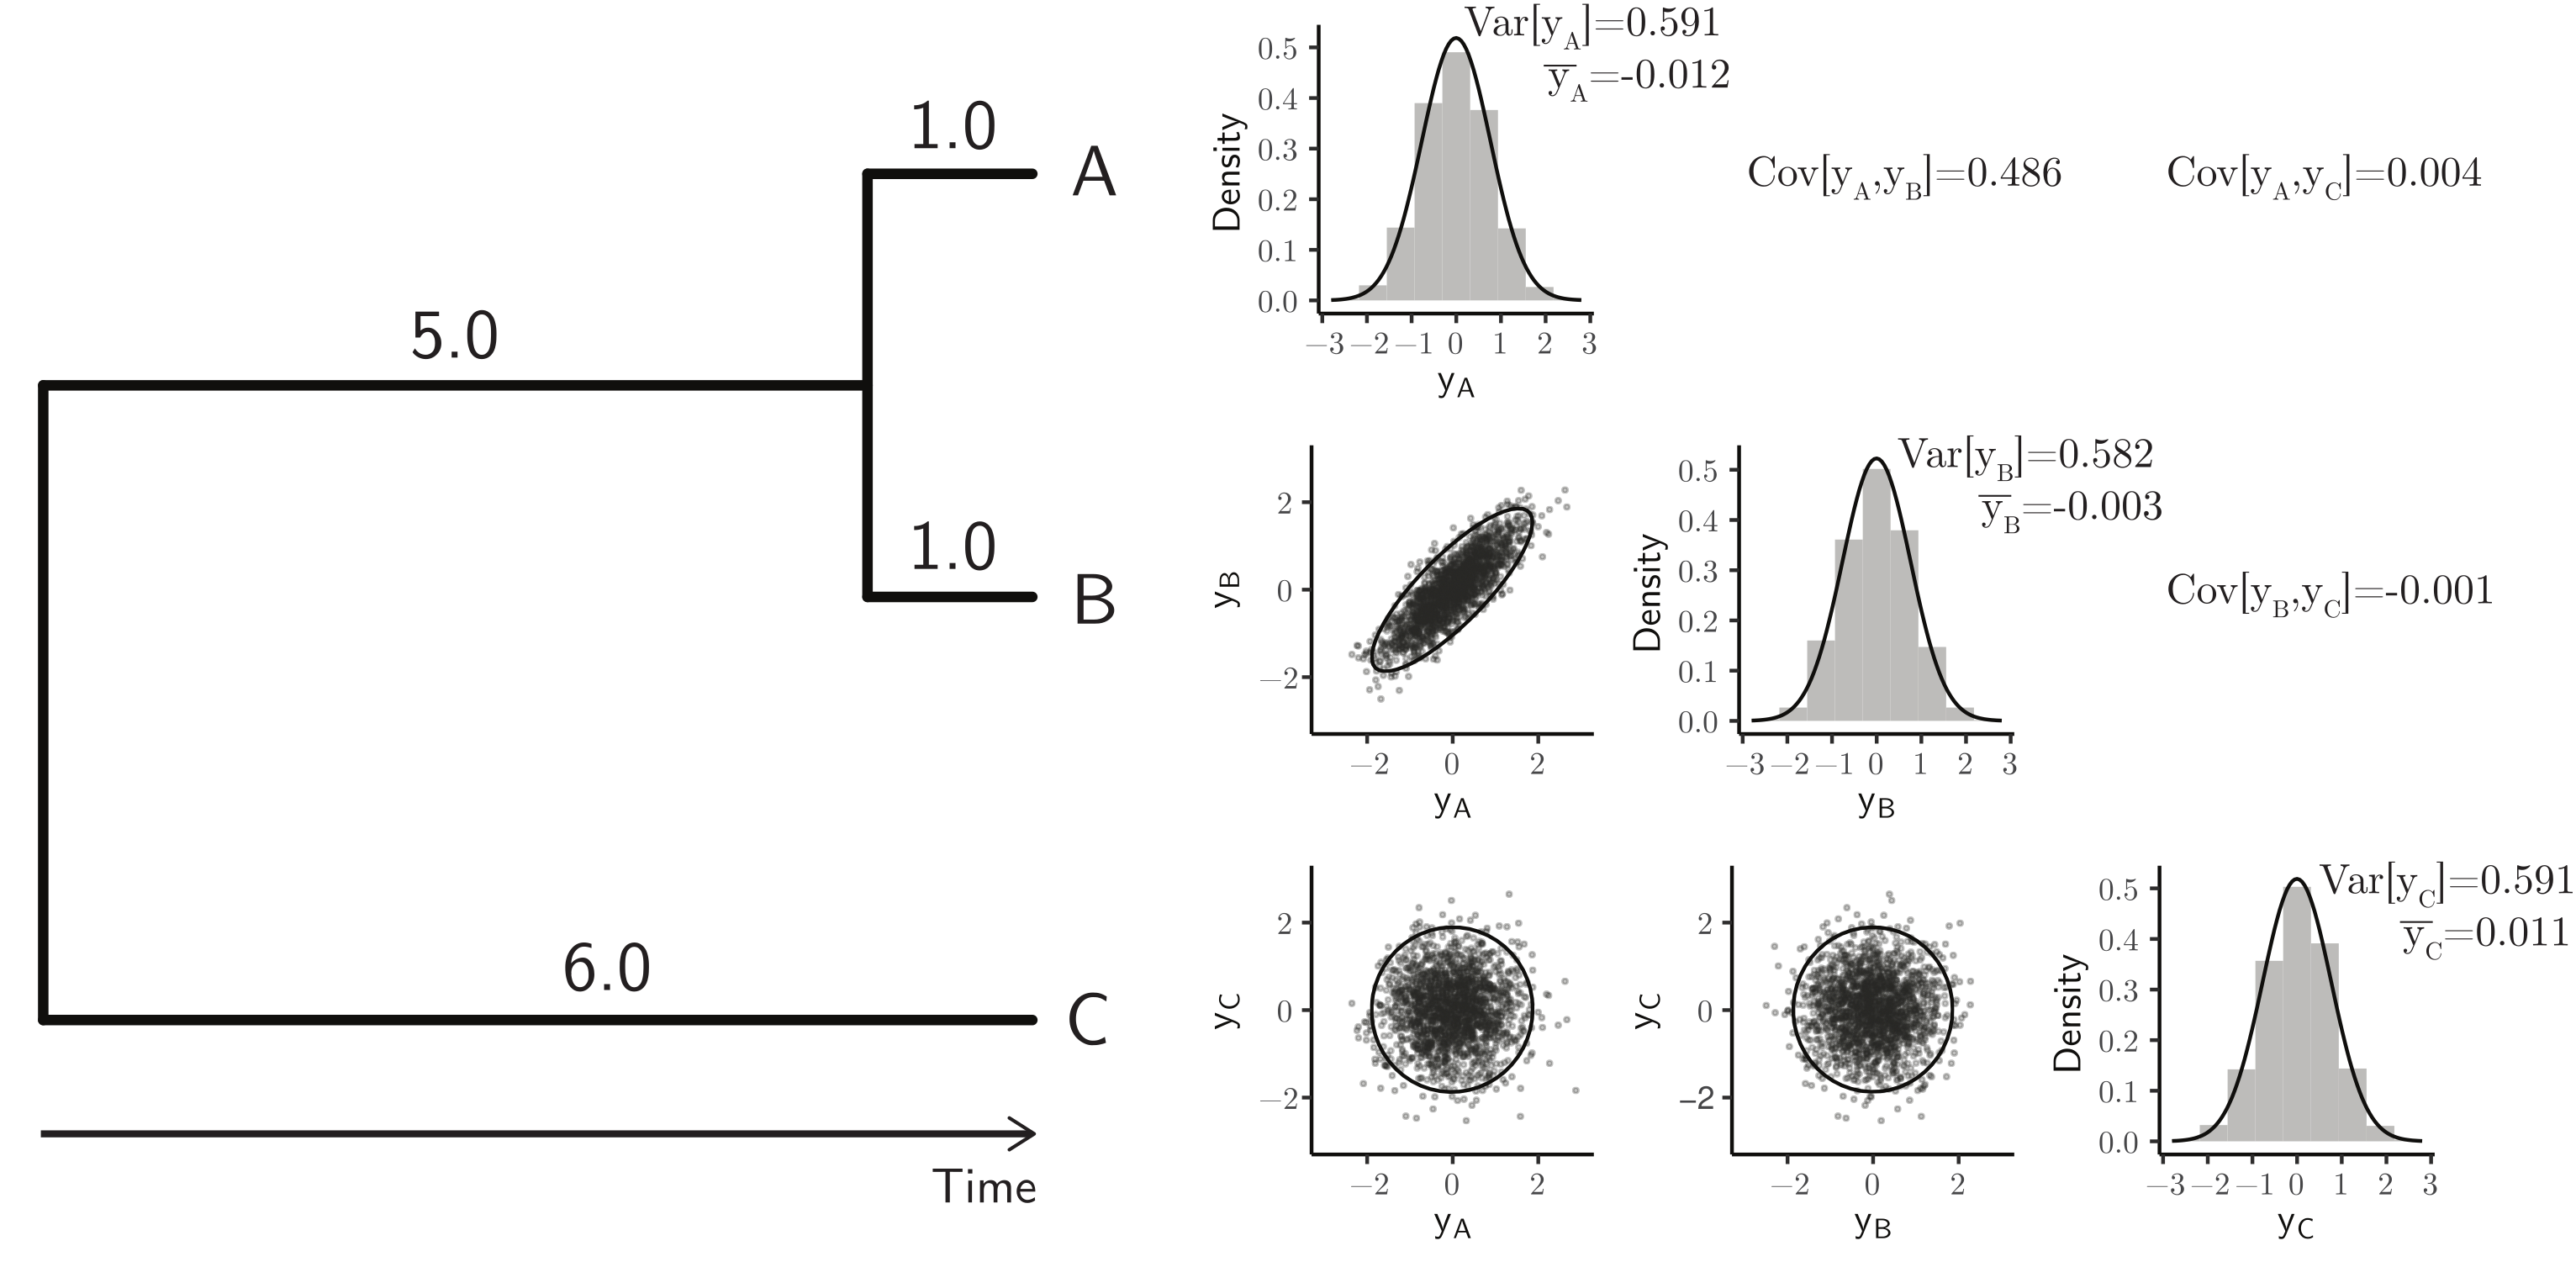
\includegraphics[width=11cm]{../figures/bmsim.pdf}
\label{fig:bmsim}
\captionof{figure}{A sample of 200 draws from a MVN distribution, each
  representing the evolutionary trajectory of one continuous trait along
  the species tree on the left. The root trait value, $\boldsymbol{y_0}$, and the
  evolutionary rate of the process, $r$, were set to 0.0 and 0.1, respectively. The panel on the right shows
  histograms of trait values sampled from the MVN for each species, as
well as their covariation.}
\end{center}

\vspace{.25cm}
\emph{Validating a phylogenetic BM simulator}

Because the MVN is a \textbf{known parametric
  distribution}, it is trivial to verify the correctness of a
phylogenetic BM model simulator, $S[f(\mathbf{y}|\boldsymbol{y_0},r,\boldsymbol{T})]$.
Figure 1 shows the result of 200 simulations under the MVN
with $\boldsymbol{y_0} = [0.0, 0.0, 0.0]$, $r = 0.1$, along the tree shown on
the left, which determines the variance-covariance matrix:
\begin{equation}
  r\boldsymbol{T} = 0.1
  \begin{bmatrix}
    6 & 5 & 0\\
    5 & 6 & 0\\
    0 & 0 & 6
  \end{bmatrix}
  \label{eq:mat}
\end{equation}

One can then verify that the simulated mean trait values and their
variances in each species fall within their 95\% confidence intervals
95\% of the time.
More specifically (i) $\boldsymbol{y_{\text{A}}}$, $\boldsymbol{y_{\text{B}}}$ and 
$\boldsymbol{y_{\text{C}}}$ fall within $[]$ X, Y and Z times out of 200, and 
(ii) $\text{Var}[\boldsymbol{y_{\text{A}}}]$,
$\text{Var}[\boldsymbol{y_{\text{B}}}]$ and
$\text{Var}[\boldsymbol{y_{\text{C}}}]$ 
fall within $[]$ X, Y and Z times out of 200.
%
%\vspace{.25cm}
%\emph{Validating a phylogenetic BM likelihood implementation}
%
% For a small tree, the likelihood of a set
% of parameter values $\theta$ given some observed data is
% straightforward to compute (following Eq. \ref{eq:bm}) and can be compared to
% the output of a focal implementation.
% Interestingly, the likelihood of the BM model can also be computed using a
% dynamic-programming algorithm known in the phylogenetics literature
% as the ``pruning'' or ``peeling'' algorithm \citep{felsenstein73}.
% Thus, if a BM model is implemented correctly, the resulting likelihood
% of $\theta$ should match the solution of equation 2 no matter
% which algorithm is used.
\end{tcolorbox}
% End: BM BOX

Another example is the Yule model (also known as the pure-birth model;
\citealt{yule24}), a continuous-time Markov process that has been
classically employed in phylogenetics to model the number of
species in a clade \citep{yule24,aldous01}.
Under a Yule process with a species birth rate of $\lambda$, the
expected tree height, $\text{E}[t_{\text{root}}]$, for
a tree with $n$ tips is:

\begin{equation}
  \text{E}[t_{\text{root}}] = \sum_{i=2}^{n}\frac{1}{1\lambda}.
  \label{eq:yule}
\end{equation}

\noindent One can then verify if $\text{E}[t_{\text{root}}]$ is $95\%$
of the time within $\pm 1.96$ standard errors of the average Yule-simulated tree
height.
Confirming that this is the case indicates $S[f(\Phi|\lambda)]$ is correctly
implemented (Fig. \ref{fig:yulemean}).

\begin{figure}
  \centering
  \vspace{0pt}
  \begin{subfigure}[t]{0.5\textwidth}
    \caption{}
    \centering
    \begin{tabular}{ c|c }
    \hline
    Birth rate ($\lambda$) & E[$t_{\text{root}}$] $\in$ 95\% CI (\%)\\
    \hline  
    0.5 & 94\\
    0.6 & 91\\
    0.7 & 98\\
    0.8 & 95\\
    0.9 & 96\\
    1.0 & 92\\
    \hline
  \end{tabular}
  \end{subfigure}
  \vspace{0pt}
  \hspace{1cm}
  \begin{subfigure}[t]{0.4\textwidth}
    \caption{}
    \centering
    \includestandalone[width=7cm]{../figures/yule_exp_height}    
  \end{subfigure}
  \hfill
  %LM TODO: think about uncertainty intervals for coverage.
  \caption{Validation of Yule tree simulator.
    (a) Number of simulated data sets (out of 100) for which the
    expected tree height ($t_{\text{root}}$) was inside the 95\% CI
    about its sample average.
    Each data set consisted of 50 twenty-taxon simulated Yule trees.
    (b) The area shaded in light blue represents the
    95\% confidence interval about the average tree height, obtained
    from the 5,000 Yule trees simulated in (a). Simulations were
    carried out with the \texttt{TreeSim} R package \citep{stadler11}.}
  \label{fig:yulemean}
\end{figure}

We note that $S[\mathcal{M}]$ represents a \emph{direct} simulator under
model $\mathcal{M}$ (Table \ref{tab:sim}), meaning each and every sample
generated by $S[\mathcal{M}]$ is
independent.
This is contrast with other simulation strategies, such as conducting
MCMC under model $\mathcal{M}$ with no data, given specific parameter
($\boldsymbol{\theta}$) values.
This latter approach may be the only option if $S[\mathcal{M}]$ has not
been yet implemented, and it is predicated upon the existence of correct
implementations of both an inferential engine $I[\mathcal{M}]'$ and of
proposal functions.
We distinguish $I[\mathcal{M}]'$ from $I[\mathcal{M}]$ because
simulations are being carried out precisely to validate $I[\mathcal{M}]$.
Unless MCMC simulations are done with $I[\mathcal{M}]'$ -- an independent
implementation of $I[\mathcal{M}]$ -- they can introduce circularity 
to the validation task.

\begin{center}
  \begin{table}
  \caption{A non-exhaustive list of direct simulation software commonly used in evolutionary
    biology analyses.}
  \label{tab:sim}
  \centering
  \begin{tabular}{ p{0.7in} | p{1.3in} | p{1in} | p{1.1in} }
    \hline
    Software package & Model type & Platform & Reference \\
    \hline  
    Seq-Gen & Molecular sequence evolution models & Standalone & \citealp{rambaut97} \\
    ms & Coalescent model & Standalone & \citealp{hudson02}\\
    SLiM & Population genetic models & Standalone & \citealp{haller19}\\
    TreeSim & Birth-death models & R & \citealp{stadler11}\\
    mvMORPH & Continuous trait evolution models & R &
                                                      \citealp{clavel15}\\
    phytools & Several phylogenetic models & R & \citealp{revell12}\\
    MASTER & Continuous-time Markov (tree) models & BEAST 2 & \citealp{vaughan13}\\
    \hline
  \end{tabular}
  \end{table}
\end{center}

% If we determine $S(M)$ samples $\text{P}_{\text{S}}(\theta)$ directly (i.e.,
% there is no data $D$; ``S'' for \textbf{s}imulation), then $I(M)$
% samples $\text{P}_{\text{I}}(\theta)$ (``I'' for \textbf{i}nference),
% and we ultimately want $\text{P}_{\text{I}}(\theta)$ to reach
% stationarity at $\text{P}_{\text{S}}(\theta$) (see box 2). 

% \begin{tcolorbox}[breakable, width=12cm, colback=gray!10, boxrule=0pt,
%   break at=11cm/0cm, title=Box 1: Models with well-known parametric \emph{pdf}'s, fonttitle=\bfseries]

% To verify correctness of a simulator implementation \(S\) for model
% \(M\) directly, the distributions \(p_S(\theta|M)\) should match
% expected distribution based on theory. We can verify this by drawing a
% large number of samples using \(S\), calculate summary statistics on the
% sample and compare these with analytical estimates for these statistics.
% For example, for tree priors, expected tree heights can often be determined, and for parametric distributions we often know mean and variance values. Simulating values and making sure the expected value is in the expected range is easy to verify in Tracer: the expected values should be within the mean value logged plus/minus 2 times stderr of mean (as shown in the summary statistics panel).

% When no analytical estimates of statistics are available, it may be possible to find a simplified case (e.g. by leaving out any trees) which can be done analytically.

% Some examples of direct simulators (this list is far from exhaustive):

% \begin{itemize}
% \item
%   the \href{http://tgvaughan.github.io/MASTER/}{MASTER} (\cite{vaughan2013stochastic}) 
%   BEAST 2 package is a general purpose package for
%   simulating stochastic population dynamics models which can be
%   expressed in terms of a chemical master equation.
% \item
%   SimSnap for SNAPP (\cite{bryant2012inferring}) is a custom build
%   implementation in C++ for simulating alignments for a fixed tree and
%   SNAPP parameters.
% \item
%   The \texttt{beast.app.seqgen.SequenceSimulator} class in BEAST 2 can
%   be used to simulate alignments for general site models using
%   reversible substitution models. See
%   \href{https://github.com/CompEvol/beast2/blob/master/examples/testSeqGen.xml}{testSeqGen.xml}
%   for an example.
% \item
%   Models implemented in other phylogenetic software packages, such a
%   BEAS 1, MrBayes, RevBayes, allow sampling a distribution using MCMC.
% \item
%   The \texttt{beast.core.DirectSimulator} class in BEAST 2 can be used
%   to draw samples from distributions in BEAST that extend
%   \texttt{beast.core.distribution.Distribution} and implement the
%   \texttt{sample(state,\ random)} method. You can set up an XML file and
%   run it in BEAST. Here are a few examples:
%   \href{https://github.com/CompEvol/beast2/blob/master/examples/testDirectSimulator.xml}{testDirectSimulator.xml},
%   \href{https://github.com/CompEvol/beast2/blob/master/examples/testDirectSimulator2.xml}{testDirectSimulator2.xml},
%   and
%   \href{https://github.com/CompEvol/beast2/blob/master/examples/testDirectSimulatorHierarchical.xml}{testDirectSimulatorHierarchical.xml}.
% \end{itemize}

\subsubsection*{Validating the inferential engine, $I(M)$}

\noindent \emph{Well-calibrated validation study}

\textcolor{red}{FKM will fill this section.}

\cite{Talts2018} propose.
PROOF of posterior CIs

\begin{table}
\begin{center}
\begin{tabular}{lc}
\hline
k & $\text{P}(x=k)$ \\ % & $\text{P}(x\le k)$ & $\text{P}(x\ge k)$\\
\hline
90 & 0.0167 \\ % & 0.0282 & 0.9718\\
91 & 0.0349 \\ % & 0.0631 & 0.9369\\
92 & 0.0649 \\ % & 0.1280 & 0.8720\\
93 & 0.1060 \\ % & 0.2340 & 0.7660\\
94 & 0.1500 \\ % & 0.3840 & 0.6160\\
95 & 0.1800 \\ % & 0.5640 & 0.4360\\
96 & 0.1781 \\ % & 0.7422 & 0.2578\\
97 & 0.1396 \\ % & 0.8817 & 0.1183\\
98 & 0.0812 \\ % & 0.9629 & 0.0371\\
99 & 0.0312 \\ % & 0.9941 & 0.0059\\
100 & 0.0059 \\ % & 1.0000 & 0.0000\\
\hline
\end{tabular}
\end{center}
\caption{Under a correctly implemented model, coverage (the number $k$
  of true simulated values that fall within their corresponding 95\%-HPDs) is binomially
  distributed, with $p=0.95$. 
\label{tab:coverage}}
\end{table}

\begin{figure}
  \includegraphics[width=\textwidth]{../figures/yule_calval.pdf}
  \caption{Calibrated validation analyses of a simple Bayesian
    hierarchical model. (a) The graphical representation of the model used in
    the analyses, where $\lambda$ is the Yule birth-rate, $n$ is the
    number of species, and $\tau$ is the set of speciation times. The
    prior is an exponential density with arbitrary mean of 0.01. Panels (b-d)
    show true $\lambda$ values plotted against their mean posteriors
    (the dashed line gives $f(x) = x$). (b) Trees
    with $50<n<200$, (c) Trees with $5<n<10$, (d) Model is
    misspecified (log-normal prior is used in inference, rather than exponential).
  }
  \label{fig:yulecalval}
\end{figure}

\noindent \emph{Simulation-based
% validation
calibration
study}

\textcolor{red}{FKM will run a SBV on a simple hierarchical model
  here.}

The basic idea is to draw $\theta^{(i)}, i = 1, \ldots, M$ from its prior, $\pi(\theta)$, simulate some data $y^{(i)}$ from $p(y^{(i)} \mid \theta^{(i)})$, use the computational machinery under evaluation to recover $p(\theta \mid y^{(i)})$ and then produce a sample $\boldsymbol\theta_s^{(i)}$ of size $L$.
Then one computes the rank $r^{(i)}$ of  $\theta^{(i)}$ in  $\boldsymbol\theta_s^{(i)}$.
\cite{Talts2018} show (Theorem 1 therein) that if the algorithm works as intended the distribution of the ranks will follow a uniform distribution on $[1, L + 1]$.

\begin{enumerate}
\setcounter{enumi}{-1}
 \item Generate a reference tree from the prior $\bar{\tau}_0  \sim \pi_T(\tau | \boldsymbol \gamma)$;
 
 \textbf{for} each iteration in 1:N, \textbf{do}:
 
 \item Generate $\bar{\tau} \sim \pi_T(\tau | \boldsymbol \gamma)$;
 \item Compute the distance $\bar{\delta} = d_\sigma(\bar{\tau},\bar{\tau}_0)$ according to the metric of choice;
 \item Generate some (aligment) data $\tilde{y} \sim p(y | \bar{\tau}, \boldsymbol\alpha)$;
 \item Draw (approximately) $\boldsymbol \tau_s = \{\tau_s^{(1)}, \tau_s^{(2)}, \ldots, \tau_s^{(L)}\}$ from the posterior $\pi(\tau | \tilde{y})$;
 \item Compute distances $\boldsymbol \delta_s = \{ \delta_1, \delta_2, \ldots, \delta_L \}$  with $\delta_i = d_\sigma(\tau_s^{(i)}, \bar{\tau}_0)$;
 \item Compute the rank $r(\boldsymbol\delta_s, \bar{\delta}) = \sum\limits_{i=1}^L \mathbb{I}(\delta_i < \bar{\delta})$.
\end{enumerate}

% Note that a tree by itself does not allow one to simulate the observables (alignments). %TODO decide whether to include this
% Obviously, one might choose to keep $\boldsymbol \alpha$ fixed during the procedure, but it this will not exactly assess the validity of the joint sampler. 
% This is particularly important for phylogenetics because the relationship between phylogeny and other parameters non-linear.

One important general point about phylogenetic space is that it does not possess a canonical representation.
The BHV parametrisation is quite useful in that allows unique geodesics and admits central limit theorems, so maybe there is some theoretical justification for using BHV path lengths as the univariate representation -- i.e. the $\delta$ -- in phylo-SBC.

\paragraph{Functionals}

The key to effective SBC is choosing functionals that reflect relevant estimators of the quantities of interest.
As with any other high-dimensional model, we explore different functionals of $\tau$ in order to study different aspects of the estimation procedure.
Unlike many models, however, phylogenies are very hard to summarise using univariate measures.
We exploit the metric nature of the space of phylogenies and compute distances with respect to a reference phylogeny $\tau_0$ under different tree distances.
In this study I have used the following functionals:
\begin{itemize}
 \item The largest branch length in $\tau$, $M(\tau)$;
 \item The length of the phylogeny, i.e.,  the sum of branch lengths $S(\tau)$;
 \item The length of the external branch leading to taxon $s_1$, $T_1(\tau)$;
 \item The Robinson-Foulds distance between $\tau$ and $\tau_0$, $\operatorname{RF}_0(\tau)$;
 \item The Billera-Holmes-Vogtman (BHV) distance between $\tau$ and $\tau_0$, $\operatorname{BHV}_0(\tau)$;
\end{itemize}

  
% There is a wide variation on the validation stringencies different
% methods and models are subjected to in the course of their
% development \citep{darriba18}.
% From a short literature review on Bayesian methods applied to
% phylogenetics (Table S1), we summarize {\color{red}{four [could be more
%     after literature review]}} main validation requirements,
% in increasing order of stringency and comprehensiveness,
% that model implementations can meet:

% \begin{enumerate}[i.]
%   \item the model produces reasonable estimates on a real data set,
%   \item the model likelihood evaluates to some theoretical
%     expectation and/or approximates an expected distribution,
%   \item the model often recovers the right parameter
%     values -- for one or more parameters (i.e., a small hand-picked
%     ``grid'' of values) -- from data sets simulated with $S(M)$, and
% \item the model correctly estimates parameter values from data sets
%   simulated from prior distributions, as indicated by the estimated
%   posterior coverage of parameters and their correlation with true
%   values (``well-calibrated validation'', see below). {\color{red}{If
%       we want to talk about the next level -- using other HPDs, we can
%       add it as the 5th possibility and expand on it below}}
% \end{enumerate}

% \vspace{.25cm}
% \noindent \emph{The model produces reasonable estimates on a real
%   data set}

% One initial yet insufficient step in validating a model implementation
% is verifying whether it produces reasonable inferences with a real
% data set.
% Depending on the particular biological question at hand, it is very
% hard or arguably impossible to know what the true, expected answer is,
% and so ``reasonable'' will always be up for debate.
% A reasonable inference could be one confirming a result from a previous study
% using the same data and model, or different data and model
% altogether, but contradictory inferences do not necessarily imply a model
% was incorrectly implemented.
% For this reason, this validation procedure cannot consist of a proper
% correctness check, but should instead be seen as an exploratory
% analysis or a sanity check (the latter would require massive
% evidence supporting a particular hypothesis).
% Accordingly, a large fraction of publications to date employ this
% strategy as a final step to illustrate the workings of a method more
% than to validate it (but see Table S1 in the supplementary material).

% \vspace{.5cm}
% \noindent \emph{The model likelihood evaluates to some
%   expected value or approximates an expected distribution}

% A good starting point in formally verifying the correctness of a
% probabilistic model implementation is the comparison between the
% likelihood of a parameter value given some data, $\text{P}(D|\theta)$, to
% some expected result.
% When models are sufficiently simple, or by focusing
% on a subcase of a complex model, it is often straightforward to derive
% what this expected result should be (see box 1).
% Using the Yule model again as an example, the probability of observing
% a phylogenetic tree $T$ given $n$ internal nodes and birth-rate
% $\lambda$ (i.e., the Yule's model likelihood function;
% \citealp{nee01}) is:

% \begin{equation}
%   \text{P}(T|n,\lambda) = (n-1)!\lambda^{n-2}e^{-\lambda L},
%   \label{eq:yulelik}
% \end{equation}

% \noindent where $L$ is the total length of the tree.
% Because likelihood functions are often computed in log-space, and
% because constants (e.g., the $(n-1)!$ term in Eq. \ref{eq:yulelik}) can be
% ignored during MCMC for efficiency, the log-likelihood function for the Yule model
% becomes:

% \begin{equation}
% \text{log P}(T|n,\lambda) = \text{log}(\lambda^{n-2}) - \lambda L.
% \end{equation}

% \noindent One can then easily compute the expected log-likelihood of an example
% tree given some $\lambda$ value by hand, and compare it against the
% value produced by the implementation being validated.
% This forms the basis of what software engineers refer to as ``unit
% testing'' (see the supplementary material for a unit test example
% under the BEAST 2 platform).
% Expected values can also be obtained from independent
% implementations of the likelihood function -- the more different the
% other implementation (e.g., different algorithms and programming
% languages are used), the more robust the test is (see box 1).

% \vspace{.25cm}
% \begin{tcolorbox}[breakable, width=\textwidth, colback=gray!10, boxrule=0pt,
%   title=Box 2: Additional validation sanity-checks, fonttitle=\bfseries]
%   \small

%   In addition to the validation procedures described in the main text,
%   method developers can opt to conduct sanity checks that will not
%   provide evidence for model correctness, but that can nonetheless
%   reveal something is wrong with the implementation of a likelihood
%   function (i.e., checks that are necessary but not sufficient).
  
%   \vspace{.25cm}
%   \emph{The score function}
  
%   One such check is looking at properties of the score function,
%   $U(\theta,D)=\frac{\partial}{\partial\theta}\log
%   \text{P}(D|\theta)$.
%   $U(\theta,D)$ is the gradient of the log-likelihood function with
%   respect to $\theta$ (the parameters in the model), thus indicating
%   the slope of $\text{P}(D|\theta)$ and its behavior given very small
%   changes in $\theta$.
%   Given a data set $D$ generated from one or more $\theta$ values, it
%   should be expected from a correct model implementation that:

%   \begin{equation}\label{eq:scorefunction}
%     \text{E}[U(\theta,D)] = \int U(\theta,D)\text{P}(D|\theta)dD = 0,
%   \end{equation}

%   This theoretical expectation can then be compared to the one
%   computed from a simulated data set (generated by $S(M)$; see the
%   supplementary material for more details).

%   \vspace{.25cm}
%   \emph{Comparing empirical vs. target posterior distributions}

%   Given a correctly implemented simulator for model $M$, $S(M)$, one
%   can directly generate a $\text{P}_{\text{S}}(\theta)$ distribution that
%   should be approximated by $\text{P}_{\text{I}}(\theta)$ at stationarity.
%   Note that under this validation scope, there is no data.
%   If chains are run long enough (as suggested by large effective
%   sample sizes, ESS's), $\text{P}_{\text{S}}(\theta)$ and
%   $\text{P}_{\text{I}}(\theta)$ can be compared, and large
%   discrepancies between them can be taken as evidence of an error in the
%   likelihood function implementation (assuming all other inferential
%   components are working properly).

%   \vspace{.15cm}
%   Such task can be done with a non-parametric test, for example, such
%   as the Kolgomorov-Smirnov test \citep{kolgomorov,smirnov,ks}, which
%   compares two empirical distribution functions (\emph{ecdf}'s) or an
%   \emph{ecdf} with a cumulative distribution function (\emph{cdf}).
%   We provide an example of this procedure in the supplementary material.
% \end{tcolorbox}

% Alternatively, a more comprehensive approach could involve comparing
% some expected quantity against its sampling distribution under the
% model being validated.
% This sampling distribution is often obtained through MCMC, with
% newly proposed parameter values being accepted in direct proportion to
% their likelihood under the model (i.e., this distribution comes from
% $I(M)$ without using any data, just a fixed $\theta$ value).
% Given a correct implementation of the Yule model,
% for example, the distribution of tree heights (for some $\lambda$
% value) should peak around the value given by from equation \ref{eq:yule}.
% This procedure is more comprehensive than unit testing because of its
% dependence on MCMC, which means a valid result requires correct
% implementations of both the likelihood function and the proposal mechanism.

% When analytical expectations are not available, the distribution
% sampled from $I(M)$ with MCMC, $\text{P}_{\text{I}}(\theta)$, can be
% compared to a target distribution sampled with $S(M)$
% ($\text{P}_{\text{S}}(\theta)$, see box 2).
% $S(M)$ can also be itself conveniently used by $I(M)$ as the proposal
% density during MCMC (see listing 2 in the supplementary material for
% an example).
% This allows isolating the validation task to the model:
% when other proposal densities are used, mismatched distributions can be
% due to malfunctioning of either or both model and proposal mechanism.

% \vspace{.5cm}
% \noindent \emph{The model often recovers the right parameter values
%   from data sets simulated at a (grid of) point(s) in parameter space}

% Perhaps the most common approach to date for validating a
% probabilistic model involves simulating data sets under specific parameter
% values -- the scope here requires a simulator $S(M)$ used to simulate
% \emph{data} under model $M$ -- carrying out inference, and tabulating
% estimates depending on how close they were to the known, true values.
% This procedure is particularly valuable in the context of point estimates
% that ignore uncertainty, characteristic of maximum-likelihood methods (e.g.,
% \citealp{mccormack09,han13,mendes17}), but of smaller if not unclear
% utility in the Bayesian framework.

% Differently from frequentist methods, which rely on approximate bootstrap
% analyses, Bayesian models allow for exact statistical inference while
% simultaneously addressing uncertainty.
% As a result, parameter estimates come in the form of a posterior
% distribution that depends not only on the model likelihood, but
% also the priors of choice.
% Validating a Bayesian model by trying to recover
% hand-picked parameter values can be problematic because it is unclear
% which prior is to be used, and also how often one should
% expect a specific highest posterior density (HPD) interval to contain
% the true parameter values.

% Presumably, correct model implementations should yield HPDs that contain
% the true values more often than not, but determining what ``often'' means
% for complex models and priors is not trivial.
% Thus, there are no theoretical guarantees that a model is correctly
% implemented should most inferred 95\% HPDs include the true parameter
% values, for example, or vice-versa.
% This validation approach can still be useful in revealing regions
% in parameter space where inference is easier or harder (given different
% prior distributions), but we instead recommend procedures that are exact,
% such as calibrated validation studies (see below).

% \vspace{.5cm}
% \noindent \emph{The model correctly estimates parameter values from
%   data sets simulated from prior distributions, as indicated by the
%   estimated posterior coverage}

% Rather than simulating a fixed number of data sets for hand-picked
% parameter values (see above), we can let the prior density of
% different values dictate how often they are used in simulations.
% This forms the basis of a calibrated validation study: a large number
% of data sets are simulated directly from the prior distributions on
% model parameters.
% Here, the choice of prior is arbitrary, but ideally should reflect
% what is currently known about the natural phenomenon being modeled.

% The advantage of this approach is that if the same Bayesian model (which
% includes likelihood \emph{and} priors) is used for both
% simulation and inference, there are clear expectations under a
% correctly implemented model.
% Namely, out of a large number of simulations, the coverage of a
% parameter should match the width of the HPD of choice
% (coverage is defined as the number of times the HPD
% interval contains the true value out of the total number of
% simulations; \citealp{dawid82}).
% For example, in the case of the commonly used 95\%-HPD interval, the true value
% should often be inside the HPD between 90--98\% of the time (Table
% \ref{tab:coverage}).


% Figure \ref{fig:yulecalval} shows the results of a calibrated
% validation analysis for a simple Bayesian model.
% Here, the full model is comprised of an exponential prior (with an
% arbitrary mean of 0.01) on the birth-rate
% $\lambda$, with the Yule likelihood (i.e., a pure-birth process)
% modelling speciation times $\tau$ (Fig. \ref{fig:yulecalval}a).
% We plot 100 ``true'' $\lambda$ values (drawn from the exponential prior)
% against their posterior means estimated through MCMC from the
% corresponding trees simulated under the Yule model
% (Fig. \ref{fig:yulecalval}b-d).
% Note that coverage is good for the first and second calibrated
% validation analyses (the vast majority of 95\%-HPDs
% include the true values, as shown by the blue vertical lines; Fig
% \ref{fig:yulecalval}b-c), for which the model was correctly
% specified.
% Coverage is not good in the third analysis, where the model was
% mispecified on purpose (a log-normal prior was used in inference,
% rather than an exponential; Fig. \ref{fig:yulecalval}d).
% Beyond coverage, one can also determine how good estimates can be,
% potentially under several simulation scenarios, by investigating the
% correlation between true parameter values and their posterior means.
% Correlation should be high when the data carries a lot of
% signal (Fig. \ref{fig:yulecalval}b), and low otherwise (Fig. \ref{fig:yulecalval}c).

% Calibrated validation is a multifarious
% analysis, as it not only verifies the correctness of a model
% likelihood (both $S(M)$ and $I(M)$), but also of all the components
% involved in the sampling of the posterior.
% For this reason, calibrated validation is the most thorough,
% integrated procedure one can carry out when the goal is to verify
% implementation correctness.
% We provide further guidelines and code examples for
% calibrated validation in the supplementary material.

\subsection*{Validating the MCMC transition mechanism (operators)}

At the heart of MCMC as an approach to sample a target distribution
(conventionally, $\text{P}(\theta|D)$) is
the Metropolis-Hastings algorithm \citep{metropolis53,mh}.
This algorithm uses a transition mechanism (i.e., a set of
``operators'') characterized by a proposal density $q(\theta'|\theta)$
that perturbs parameter values $\theta$ toward new values $\theta'$.
The Markov chain progresses as these perturbations are accepted, which
occurs with probability $\alpha$:

\begin{equation}
  \alpha = \text{min}\bigg(1, \frac{\text{P}(\theta'|D)}{\text{P}(\theta|D)} \frac{q(\theta|\theta')}{q(\theta'|\theta)} \bigg),
\end{equation}

\noindent where $\frac{q(\theta|\theta')}{q(\theta'|\theta)}$ is also
referred to as the Hastings ratio \citep{smith93,tierney94,gelman}.
For simple proposal densities, the Hastings ratio will often be unity and
only the prior and likelihood ratios must be computed.
It is sometimes the case, however, that more complex proposals will
increase or reduce the dimensionality of parameter space, in which
case the derivation of the Hastings ratio will be less straightforward.
For the sake of brevity, we point the reader to the relevant theory
and examples in \citep{green95,huelsenbeck04,drummond10}.

Although operators are not strictly part of the model (as mentioned
above, MCMC is not the only way to sample or approximate a target
distribution), it is absolutely vital to validate them prior or
together with the model per se, should MCMC be the approach of choice.
Only correctly implemented operators will lead to ergodic (i.e.,
irreducible, positive recurrent, and aperiodic) Markov
chains with a stationary distribution that will hopefully match
the target distribution, should the chain be long enough.

In the context of MCMC, unless a direct simulator $S(M)$ is
available to be used as a proposal mechanism (see above), model and operator
validation can be seen as two sides of the same coin.
Outside of unit-testing, validating models requires carrying out MCMC
(see items (ii) and (iv) in the previous section, for example), which
in turn can only be a meaningful procedure if correctly implemented
operators are available.
Conversely, if the intention is to validate new operators, then a
model under which to evaluate proposals must have been correctly
implemented prior to MCMC.

In the latter case, the principle behind validation is the same: one
compares the stationary distribution (with respect to one or more summary
statistics) obtained using the operator(s)
being tested, $\text{P}_{\text{I}}(\theta)$, with an expected
distribution, $\text{P}_{\text{S}}(\theta)$ (see listing 5 in
supplementary material). 
This second, expected distribution can be obtained through MCMC with a
mutually exclusive set of correctly implemented operators capable of
generating an ergodic chain (see item
(a) in supplementary table S1). 

Finally, a well-calibrated validation study also serves the purpose of
validating the transition mechanism.
Low coverage might indicate not only that the model was incorrectly
implemented, but also that operators are not functioning as expected.
Determining which of the two possibilities -- or whether both are
happening -- is not a trivial task, and careful diagnostics are
necessary on the part of method developers.

\section*{Concluding remarks}

As more data is generated and made publicly available, the more will
researchers in the life sciences require computational methods with
which to analyze it.
If such methods are not correctly implemented, conclusions drawn from
the data will be of reduced or void of any significance.
Here we discuss guidelines for the validation of computational methods
implementing Bayesian probabilistic models.
This manuscript is also followed by a supplementary text further
illustrating these guidelines that is linked with a live document
available on \href{https://github.com/rbouckaert/DeveloperManual}{https://github.com/rbouckaert/DeveloperManual}.
We hope our guidelines can help raise the standards for software
package releases required by users, developers and reviewers alike,
and consequently lead to computational tools that are more efficient,
better documented, and most importantly, correctly implemented.

\subsection*{Funding}
F.K.M. and A.J.D. were supported by Marsden grant 16-UOA-277. R.B. was
supported by Marsden grant .


%----------------------------------------------------------------------------------------
%	REFERENCE LIST
%----------------------------------------------------------------------------------------

% \section*{References}
% \clearpage

\bibliography{refs}

%----------------------------------------------------------------------------------------

\end{document}
